\documentclass[12pt]{article}
\usepackage[utf8]{inputenc}
\usepackage{graphics}
\usepackage{graphicx}
\usepackage{float}
\usepackage{hyperref}
\usepackage{listings}
\lstset{
	basicstyle=\ttfamily,
	columns=fullflexible,
	frame=single,
	breaklines=true,
	postbreak=\mbox{\textcolor{red}{$\hookrightarrow$}\space},
}
\hypersetup{
	colorlinks=true,
	linkcolor=blue,
	filecolor=magenta,      
	urlcolor=cyan,
}

\title{De kwaliteit automatisch controleren}
\author{Thomas van Dongen, Koen Schilders}
\date{11 april 2018}

\begin{document}


% De titelpagina
\begin{titlepage}
\maketitle
\end{titlepage}

\section{Inleiding}
Voor deze opdracht gaan we SonarQube toevoegen aan de ontwikkelstraat om de kwaliteit van de code grondig te testen. Dit gebeurt met SonarQube, een open source platform voor het statisch testen van code.

\section{SonarQube docker}
SonarQube zal in een eigen docker container draaien. Dit hoeven we niet zelf op te zetten: hier is namelijk een image van:
\begin{lstlisting}[language=Bash]
docker pull sonarqube
\end{lstlisting}

Nu kunnen de sonarqube container draaien:
\begin{lstlisting}[language=Bash]
docker run -d --name sonarqube -p 9000:9000 -p 9092:9092 sonarqube:latest
\end{lstlisting}

SonarQube draait op poort 9000. We kunnen controleren of SonarQube draait door naar localhost:9000 te gaan. Hier kunnen we inloggen met admin als gebruikersnaam en admin als wachtwoord. In SonarQube moeten we een token genereren. Deze token hebben we nodig in Jenkins.

\begin{figure}[H]
	\begin{center}
		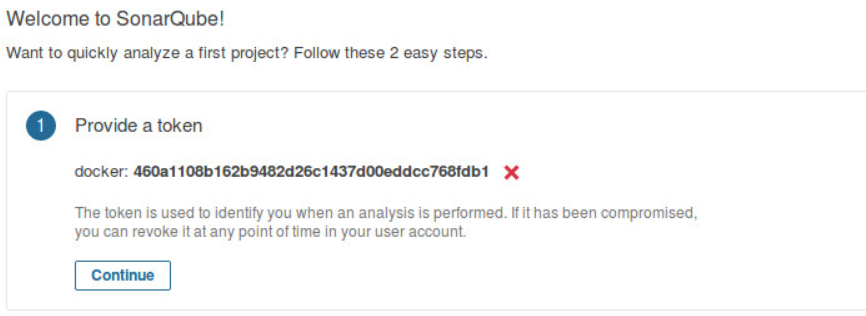
\includegraphics[width=0.75\textwidth]{images/sonarqube_token.PNG}
		\caption{De SonarQube token\label{fig:sonarqube_token}}
	\end{center}
\end{figure}


\section{SonarQube Scanner}
Nu moeten we Jenkins laten weten waar de SonarQube server te vinden is, waarvoor we de SonarQube Scanner plugin gebruiken. Dit moet in Jenkins - Configuratie - SonarQube servers. Het is belangrijk om localhost:9000 te vervangen door IP:9000, in ons geval 192.168.24.125:9000. Vul de token in van de vorige stap. Nu kan Jenkins de SonarQube server vinden.

\begin{figure}[H]
	\begin{center}
		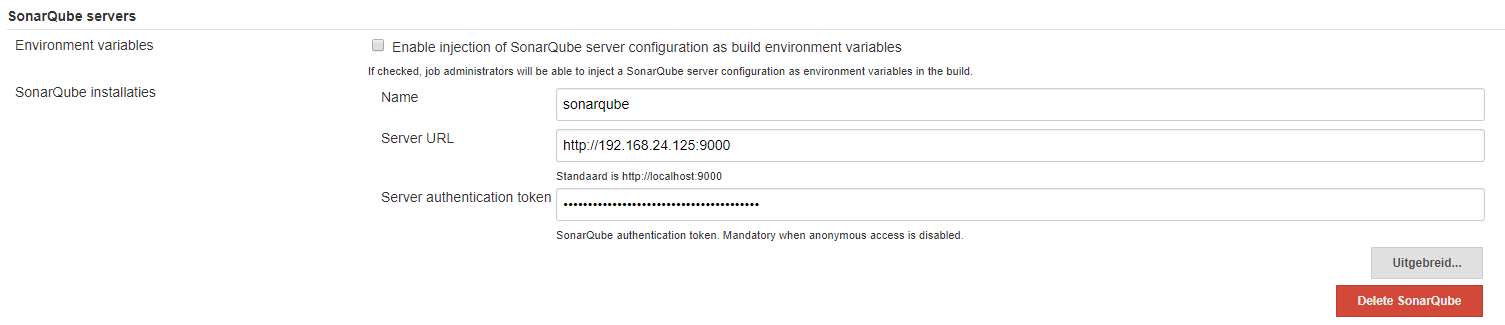
\includegraphics[width=0.75\textwidth]{images/sonarqube_instellen_jenkins.PNG}
		\caption{SonarQube instellingen\label{fig:sonarqube_instellen_jenkins}}
	\end{center}
\end{figure}

Jenkins kunnen we nu met een bouwstap toevoegen aan de ontwikkelstraat. SonarQube Scanner heeft enkele settings nodig om succesvol SonarQube uit te voeren. Zo moet de plugin weten wat de logingegevens en projectnaam zijn, en welke bestanden hij moet testen.

\begin{figure}[H]
	\begin{center}
		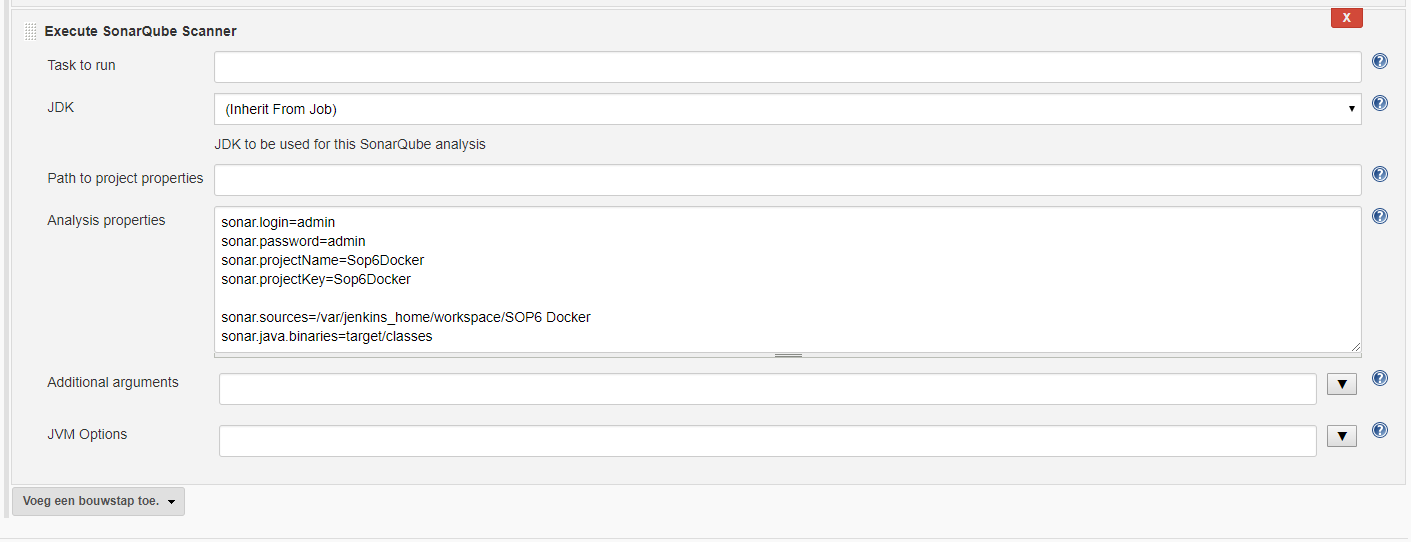
\includegraphics[width=0.75\textwidth]{images/jenkins_configuratie.png}
		\caption{Jenkins configuratie\label{fig:jenkins_configuratie}}
	\end{center}
\end{figure}

Na het configureren kan een nieuwe bouwpoging gestart worden. In de logs is te zien dat SonarQube succesvol uitgevoerd wordt. In het overzicht van het Jenkins project is ook te zien dat SonarQube succesvol uitgevoerd is.

\begin{figure}[H]
	\begin{center}
		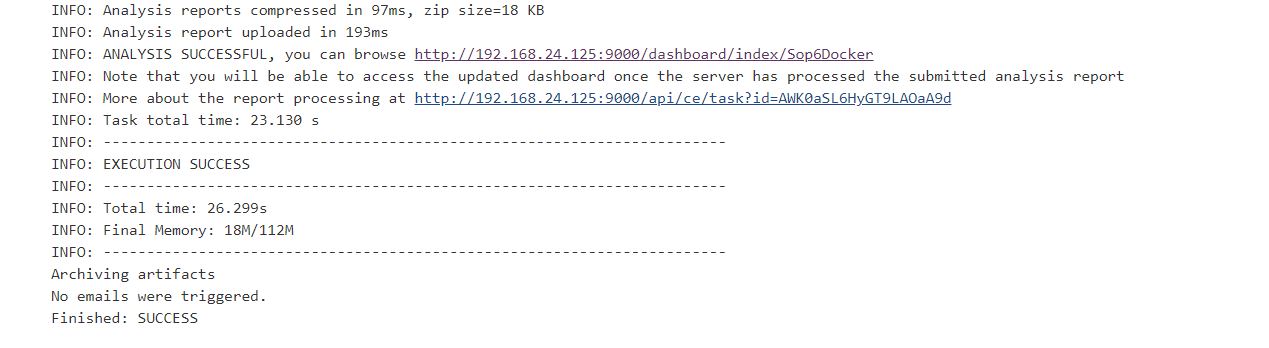
\includegraphics[width=0.75\textwidth]{images/succes.PNG}
		\caption{De output van een build\label{fig:succes}}
	\end{center}
\end{figure}

\begin{figure}[H]
	\begin{center}
		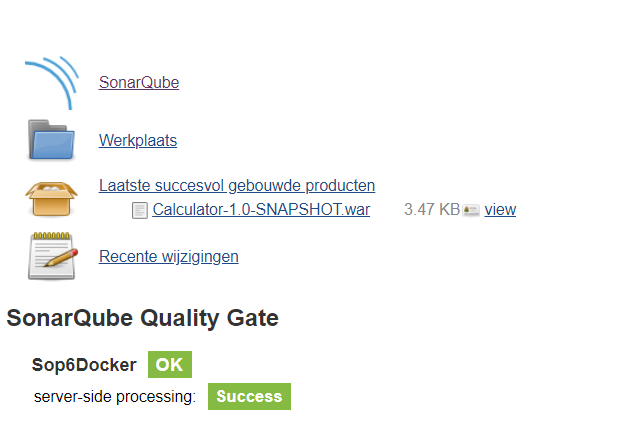
\includegraphics[width=0.75\textwidth]{images/overzichtjenkins.PNG}
		\caption{Overzich in Jenkins project\label{fig:overzichtjenkins}}
	\end{center}
\end{figure}

In de SonarQube dashboard kan de uitslag nader bekeken worden. Zo heeft het testproject 5 Code Smells, waar mogelijk naar gekeken moet worden.

\begin{figure}[H]
	\begin{center}
		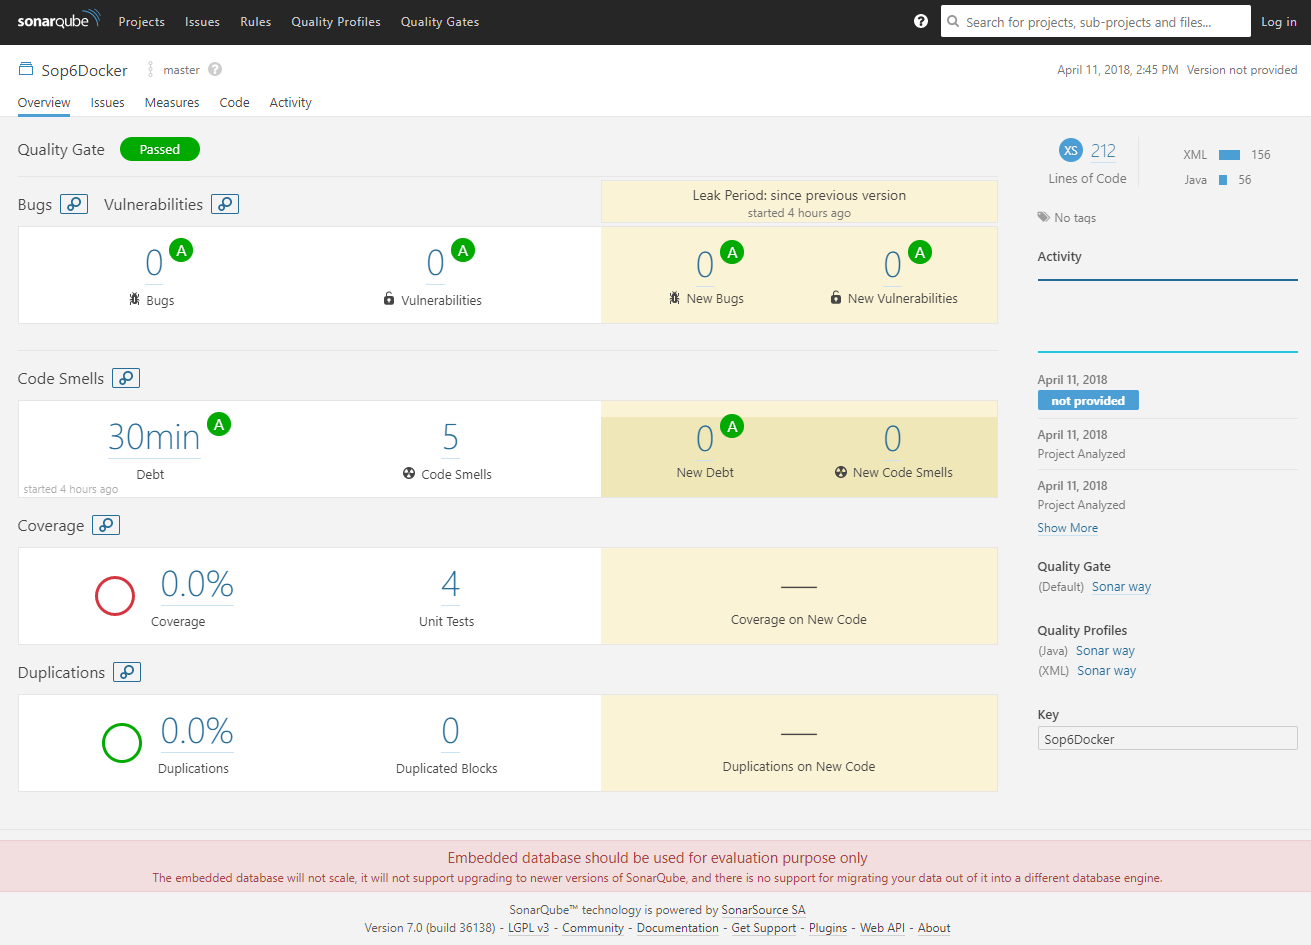
\includegraphics[width=0.75\textwidth]{images/sonarqube_dashboard.png}
		\caption{Het dashboard van SonarQube\label{fig:succes}}
	\end{center}
\end{figure}


% Sources
\begin{thebibliography}{9}
	\bibitem{sonarqube_scanner_plugin}
	Jenkins,
	\textit{SonarQube Scanner},
	\url{https://plugins.jenkins.io/sonar}
\end{thebibliography}

\end{document}